\documentclass[11pt]{amsart}
\usepackage[margin=1.1in]{geometry}
\usepackage{amssymb,mathtools}
\usepackage{graphicx}
\usepackage[hidelinks]{hyperref}
\usepackage{doi}

\newtheorem{theorem}{Theorem}[section]
\newtheorem{lemma}[theorem]{Lemma}
\newtheorem{proposition}[theorem]{Proposition}
\newtheorem{corollary}[theorem]{Corollary}
\newtheorem*{theoremA}{Theorem A}
\newtheorem*{theoremB}{Theorem B}
\newtheorem*{theoremC}{Theorem C}
\theoremstyle{definition}
\newtheorem{definition}[theorem]{Definition}
\newtheorem{example}[theorem]{Example}
\theoremstyle{remark}
\newtheorem{remark}[theorem]{Remark}

\newcommand{\R}{\mathbb{R}}
\newcommand{\Z}{\mathbb{Z}}
\newcommand{\J}{\mathfrak{J}}
\newcommand{\qa}{\vdash}
\newcommand{\supp}{\operatorname{supp}}
\newcommand{\up}{{\uparrow}}
\newcommand{\dn}{{\downarrow}}

\begin{document}

\title{The Aperiodic Jordan Algebras of Quasicrystals Are Not Jordan}

\author{Deep Bhattacharjee}
\address{Formerly, Electro-Gravitational Space Propulsion Laboratory (EGSPL), Bhubaneswar, Odisha 751030, India}
\address{Formerly, University of Calcutta (Heramba Chandra College), 23/49 Gariahat Road, Golpark, Kolkata 700029, West Bengal, India}
\email{d.bhattacharjee@erl-forschung.de}
\email{itsdeep@live.com}
\email{egspl@proton.me (GitHub-related contact; GitHub: creelie)}
\urladdr{https://orcid.org/0000-0003-0466-750X}

\subjclass[2020]{17C05, 17A05, 52C23}
\keywords{Jordan algebras, power-associative algebras, quasicrystals}

\begin{abstract}
Corradetti, Chester, Aschheim and Irwin attached to every quasicrystal closed under quasiaddition an algebra with product $L_x\circ L_y=\frac12(L_{x\vdash y}+L_{y\vdash x})$ and stated that it is a Jordan algebra. It is not even power-associative: $x^2x^2=x^3x$ holds exactly when $x$ is a multiple of a generator.
\end{abstract}

\maketitle

\section{Introduction}

Quasicrystal Lie algebras were introduced by Patera, Pelantov\'a and Twarock \cite{PPT98}: their generators $L_x$ are indexed by the points $x$ of a one-dimensional quasicrystal, and the bracket $[L_x,L_y]$ is a multiple of $L_{x+y}$ when $x+y$ lies again in the quasicrystal and vanishes otherwise. Corradetti, Chester, Aschheim and Irwin replaced the sum by the \emph{quasiaddition} of Berman and Moody \cite{BM94},
\begin{equation}\label{eq:qa}
x\qa y=\tau^2x-\tau y,\qquad \tau=\tfrac{1+\sqrt5}{2},
\end{equation}
under which every model set with a convex window is closed, and defined on the span of the generators the commutative product
\begin{equation}\label{eq:product}
L_x\circ L_y=\tfrac12\left(L_{x\qa y}+L_{y\qa x}\right).
\end{equation}
In \cite[Section~5]{CCAI23} this is done for the Fibonacci-chain quasicrystals and the resulting algebra is called ``the first aperiodic Jordan algebra''; in \cite[Section~5]{CCAI25} the same product is placed on every icosahedral model set with a convex window, in dimensions one to four, and a theorem states that the algebra is a Jordan algebra. Both papers go on to derive structural properties from the Jordan property, and \cite{CCAI23} proposes, through Svinolupov's correspondence between Jordan algebras and integrable systems of Korteweg--de Vries type \cite{Svi91}, an application of finite truncations of the algebra to solitons.\footnote{We quote the arXiv versions arXiv:2302.04044 and arXiv:2303.12219 of \cite{CCAI23,CCAI25}. In \cite{CCAI23} the claim is the construction of Section~5 together with its Conclusions; in \cite{CCAI25} it is the first theorem of Section~5.}

The proof given in both papers checks the Jordan identity
\begin{equation}\label{eq:jordan}
(x\circ y)\circ(x\circ x)=x\circ\bigl(y\circ(x\circ x)\bigr)
\end{equation}
for $x=L_p$ and $y=L_q$, using $p\qa p=p$. Since \eqref{eq:jordan} is cubic in $x$, its validity on a basis says nothing about sums of basis vectors; a check on generators would have to be made on the full linearisation of the identity \cite[Part~II]{McC04}. We show that the identity fails for every element outside the lines spanned by the generators. Throughout, $\Xi$ is a subset of a real vector space $V$ that is closed under \eqref{eq:qa} and has at least two points, and $\J(\Xi)$ is the real vector space with basis $\{L_x\}_{x\in\Xi}$ and product \eqref{eq:product}. We write $x^2=x\circ x$ and $x^3=x^2\circ x$.

\begin{theoremA}
For $x\in\J(\Xi)$ the following are equivalent.
\begin{enumerate}
\item[(i)] $x=cL_p$ for some $c\in\R$ and $p\in\Xi$.
\item[(ii)] The Jordan identity \eqref{eq:jordan} holds for $x$ and every $y\in\J(\Xi)$.
\item[(iii)] $x^2\circ x^2=x^3\circ x$.
\end{enumerate}
In particular $\J(\Xi)$ is neither a Jordan algebra nor a power-associative algebra.
\end{theoremA}

A Jordan algebra is power-associative \cite{Alb48,McC04}, and in a commutative algebra power-associativity in degree four is exactly (iii); so Theorem~A shows that $\J(\Xi)$ already fails the weakest consequence of the Jordan identity, and that the computation in \cite{CCAI23,CCAI25}, which is the implication (i)$\Rightarrow$(ii), is the whole range in which the identity holds. The cases covered include every Fibonacci-chain quasicrystal $\mathcal F_{\alpha,\beta}$ of \cite{CCAI23} and the Fibonacci chain, the Penrose tiling and the Elser--Sloane quasicrystal of \cite{CCAI25}. For $x=L_1+L_{1+\tau}$ in the Fibonacci chain $\mathcal F_{1,0}$ the generator $L_{9+13\tau}$ occurs in $x^3\circ x$ with coefficient $\frac14$ and does not occur in $x^2\circ x^2$ (Example~\ref{ex:fibonacci} and Figure~\ref{fig:supports}).

The finite algebras proposed in \cite[Section~6]{CCAI23} are obtained by keeping finitely many consecutive points of the chain and setting a product to zero when a quasiaddition leaves them; \cite{CCAI23} states that commutativity and the Jordan identity survive this truncation.

\begin{theoremB}
Truncation does not produce Jordan algebras. Keeping the three consecutive points $1$, $1+\tau$, $2+2\tau$ of $\mathcal F_{1,0}$ gives the three-dimensional commutative algebra with basis $e_1,e_2,e_3$ and products $e_i^2=e_i$, $e_1e_2=\frac12e_3$, $e_1e_3=e_2e_3=0$, in which $x=e_1+e_2$ satisfies $x^2x^2-x^3x=e_3$. More generally, for every $x\in\J(\Xi)$ with at least two points in its support there is a finite set $T\subset\Xi$ such that every truncation to a finite set $S\supseteq T$ fails power-associativity.
\end{theoremB}

Finally we examine the structural statements that \cite{CCAI23,CCAI25} derive for these algebras.

\begin{theoremC}
\begin{enumerate}
\item[(a)] The subspace $\mathfrak k=L_1\circ\J(\mathcal F_{1,0})$, which \cite{CCAI23} uses as a proper ideal to show that $\J(\mathcal F_{1,0})$ is not simple, is not an ideal: $(L_1\circ L_{1+\tau})\circ L_{2+3\tau}\notin\mathfrak k$.
\item[(b)] Nevertheless $\J(\Xi)$ is not simple: the coefficient sum is a nonzero algebra homomorphism $\J(\Xi)\to\R$.
\item[(c)] $\J(\Xi)$ has no unit, its one-dimensional subalgebras are the lines $\R L_x$, and it has no finite-dimensional subalgebra of dimension at least two.
\item[(d)] No algebra containing $\J(\Xi)$ as a subalgebra is a Jordan algebra; in particular the unital extension of $\J(\Xi)$ described in \cite[Section~5]{CCAI25} is not one.
\end{enumerate}
\end{theoremC}

Parts (b) and (c) confirm conclusions of \cite{CCAI23,CCAI25}, but the proofs given there do not establish them: the argument for non-simplicity in \cite{CCAI23} rests on the subspace in (a), the arguments for the absence of a unit in both papers manipulate the infinite sum $\sum_{x\in\Xi}L_x$, which is not an element of the algebra, and the argument for the absence of finite-dimensional subalgebras in \cite{CCAI25} assumes that such a subalgebra contains two generators $L_x,L_y$.

The proofs rest on one observation. Quasiaddition commutes with affine maps, so after choosing a linear functional that separates the points of a support, each product of finitely supported elements has a highest and a lowest point whose coefficients can be read off exactly (Lemmas~\ref{lem:square} and~\ref{lem:product}). Following the highest point through $x^2$, $x^3$, $x^2\circ x^2$ and $x^3\circ x$ proves Theorem~A. Other questions raised by the construction of Rios, Marrani and Chester in a different setting are treated in \cite{Bha26,Arch}, and further algebraic invariants attached to geometric data are studied in \cite{Bha22,Bha26b}.

\section{Quasiaddition and the algebra \texorpdfstring{$\J(\Xi)$}{J(Xi)}}

Let $V$ be a real vector space and let $\tau=\frac{1+\sqrt5}{2}$, so that $\tau^2=\tau+1$. Repeated use of this relation gives
\begin{equation}\label{eq:powers}
\tau^3=2\tau+1,\quad \tau^4=3\tau+2,\quad \tau^5=5\tau+3,\quad \tau^6=8\tau+5,\quad \tau^7=13\tau+8 .
\end{equation}
Quasiaddition \eqref{eq:qa} can be written as $x\qa y=y+\tau^2(x-y)$, because $\tau^2-\tau=1$.

\begin{lemma}\label{lem:qa}
Let $x,y\in V$.
\begin{enumerate}
\item[(a)] $x\qa x=x$.
\item[(b)] If $\varphi\colon V\to W$ is an affine map into a real vector space $W$, then $\varphi(x\qa y)=\varphi(x)\qa\varphi(y)$. In particular $f(x\qa y)=\tau^2f(x)-\tau f(y)$ for every affine function $f\colon V\to\R$.
\item[(c)] $x\qa y=x$ if and only if $y=x$, and $y\qa x=x$ if and only if $y=x$.
\item[(d)] If $\Xi\subset V$ is closed under quasiaddition and contains two points $a\neq b$, then $\Xi$ is infinite.
\end{enumerate}
\end{lemma}

\begin{proof}
(a) $x\qa x=(\tau^2-\tau)x=x$. (b) Write $\varphi(v)=Av+w$ with $A$ linear. Then $\varphi(x\qa y)=\tau^2Ax-\tau Ay+w=\tau^2(Ax+w)-\tau(Ay+w)$, since $\tau^2-\tau=1$; this is $\varphi(x)\qa\varphi(y)$. (c) $x\qa y=x$ means $(\tau^2-1)x=\tau y$, that is $\tau x=\tau y$; and $y\qa x=x$ means $\tau^2y=(1+\tau)x=\tau^2x$. (d) Put $z_0=b$ and $z_{k+1}=z_k\qa a$. By the second form of \eqref{eq:qa}, $z_{k+1}-a=\tau^2(z_k-a)$, so $z_k-a=\tau^{2k}(b-a)$, and these vectors are pairwise distinct because $\tau^2>1$ and $b\ne a$. All $z_k$ lie in $\Xi$.
\end{proof}

For a subset $\Xi\subset V$ closed under quasiaddition we write $\J(\Xi)$ for the real vector space with basis $\{L_x\}_{x\in\Xi}$ and the bilinear product \eqref{eq:product}. An element is written $u=\sum_xa_xL_x$ with finitely many nonzero $a_x$; its \emph{support} $\supp u$ is the set of $x$ with $a_x\ne0$. Expanding \eqref{eq:product} bilinearly, for $u=\sum_xa_xL_x$ and $v=\sum_yb_yL_y$,
\begin{equation}\label{eq:uv}
u\circ v=\tfrac12\sum_{x,y}a_xb_y\left(L_{x\qa y}+L_{y\qa x}\right),
\end{equation}
the sum running over $x\in\supp u$ and $y\in\supp v$. When $v=u$ the two halves of \eqref{eq:uv} are exchanged by renaming $x\leftrightarrow y$, hence
\begin{equation}\label{eq:uu}
u\circ u=\sum_{x,y\in\supp u}a_xa_yL_{x\qa y}.
\end{equation}
In particular $L_x\circ L_x=L_x$ by Lemma~\ref{lem:qa}(a), and the product is commutative.

The quasicrystals of \cite{CCAI23,CCAI25} are of this kind. A Fibonacci-chain quasicrystal is $\mathcal F(\Omega)=\{n\in\Z[\tau]:n^*\in\Omega\}\subset\R$, where $\Omega$ is an interval of length one and $(n_1+n_2\tau)^*=n_1+n_2(1-\tau)$ is the Galois conjugation; the sets $\mathcal F_{\alpha,\beta}$ of \cite{CCAI23} are the cases $\Omega=(\alpha+\beta-1,\alpha+\beta]$. Since conjugation is a ring automorphism of $\Z[\tau]$ and $(1-\tau)^2-(1-\tau)=1$, it satisfies $(x\qa y)^*=(1-\tau)^2x^*-(1-\tau)y^*=y^*+(1-\tau)^2(x^*-y^*)$, and this point lies between $x^*$ and $y^*$ because $0<(1-\tau)^2<1$; so a convex window gives a set closed under \eqref{eq:qa}. The icosahedral model sets of \cite{CCAI25} in $\R^2$, $\R^3$ and $\R^4$ are closed under \eqref{eq:qa} for the same reason \cite[Section~4]{CCAI25}. We shall use only closure under \eqref{eq:qa}.

For $\mathcal F_{1,0}$, where $\Omega=(0,1]$, the points near the origin are
\[
\dots,\ -1-3\tau,\ -1-2\tau,\ -\tau,\ 1,\ 1+\tau,\ 2+2\tau,\ 2+3\tau,\ 3+4\tau,\ \dots
\]
For instance $(2+3\tau)^*=5-3\tau\in(0,1]$, while $0^*=0$ and $\tau^*=1-\tau$ are not in $(0,1]$, so $0,\tau\notin\mathcal F_{1,0}$.

\section{The leading terms of a product}

Fix an affine function $f\colon V\to\R$. For a nonzero $u=\sum a_xL_x$ put
\[
M_f(u)=\max_{x\in\supp u}f(x),\qquad m_f(u)=\min_{x\in\supp u}f(x).
\]
We call $u$ \emph{$f$-sharp} if exactly one point of $\supp u$, denoted $u^\up$, has $f(u^\up)=M_f(u)$, and exactly one point, denoted $u^\dn$, has $f(u^\dn)=m_f(u)$. Their coefficients $u_\up=a_{u^\up}$ and $u_\dn=a_{u^\dn}$ are then nonzero.

\begin{lemma}\label{lem:square}
Let $u$ be $f$-sharp with $M=M_f(u)>m=m_f(u)$. Then $u\circ u$ is $f$-sharp, with
\[
M_f(u\circ u)=\tau^2M-\tau m,\qquad m_f(u\circ u)=\tau^2m-\tau M,
\]
$(u\circ u)^\up=u^\up\qa u^\dn$ and $(u\circ u)^\dn=u^\dn\qa u^\up$, and both of these points carry the coefficient $u_\up u_\dn$. Moreover $M_f(u\circ u)-M>0$ and $M_f(u\circ u)-m_f(u\circ u)=\tau^3(M-m)>0$.
\end{lemma}

\begin{proof}
By \eqref{eq:uu} the support of $u\circ u$ is contained in $\{x\qa y:x,y\in\supp u\}$, and by Lemma~\ref{lem:qa}(b)
\[
f(x\qa y)=\tau^2f(x)-\tau f(y)\le\tau^2M-\tau m,
\]
with equality if and only if $f(x)=M$ and $f(y)=m$, that is, by sharpness, if and only if $(x,y)=(u^\up,u^\dn)$. Put $z_0=u^\up\qa u^\dn$. The coefficient of $L_{z_0}$ in \eqref{eq:uu} is the sum of $a_xa_y$ over the pairs with $x\qa y=z_0$; each such pair has $f(x\qa y)=f(z_0)=\tau^2M-\tau m$ and is therefore $(u^\up,u^\dn)$. So the coefficient is $u_\up u_\dn\neq0$, the point $z_0$ belongs to the support, and every other point $z$ of the support satisfies $f(z)<\tau^2M-\tau m$, since a point with equality would be $u^\up\qa u^\dn=z_0$. The statement about the lowest point follows in the same way from $f(x\qa y)\ge\tau^2m-\tau M$, with equality exactly for $(x,y)=(u^\dn,u^\up)$. Finally $(\tau^2M-\tau m)-M=\tau(M-m)>0$ because $\tau^2-1=\tau$, and $(\tau^2M-\tau m)-(\tau^2m-\tau M)=(\tau^2+\tau)(M-m)=\tau^3(M-m)$.
\end{proof}

\begin{lemma}\label{lem:product}
Let $u$ and $v$ be $f$-sharp, and put
\begin{align*}
A&=\tau^2M_f(u)-\tau m_f(v), & B&=\tau^2M_f(v)-\tau m_f(u),\\
a&=\tau^2m_f(u)-\tau M_f(v), & b&=\tau^2m_f(v)-\tau M_f(u).
\end{align*}
Every point $z$ of $\supp(u\circ v)$ satisfies $\min(a,b)\le f(z)\le\max(A,B)$. If $A>B$, then $u^\up\qa v^\dn$ is the only point of $\supp(u\circ v)$ with $f=M_f(u\circ v)$, this maximum equals $A$, and the coefficient of $L_{u^\up\qa v^\dn}$ in $u\circ v$ is $\frac12u_\up v_\dn$. If $a<b$, then $u^\dn\qa v^\up$ is the only point with $f=m_f(u\circ v)$, this minimum equals $a$, and its coefficient is $\frac12u_\dn v_\up$. In particular, if $A>B$ and $a<b$, then $u\circ v$ is $f$-sharp.
\end{lemma}

\begin{proof}
By \eqref{eq:uv} the coefficient of $L_z$ in $u\circ v$ is
\begin{equation}\label{eq:coef}
\tfrac12\sum_{x\qa y=z}a_xb_y+\tfrac12\sum_{y\qa x=z}a_xb_y,
\end{equation}
with $x\in\supp u$ and $y\in\supp v$ in both sums. A point of the first kind, $z=x\qa y$, satisfies $f(z)=\tau^2f(x)-\tau f(y)\le A$, with equality only for $(x,y)=(u^\up,v^\dn)$; a point of the second kind, $z=y\qa x$, satisfies $f(z)=\tau^2f(y)-\tau f(x)\le B$, with equality only for $y=v^\up$ and $x=u^\dn$. The lower bounds $f(z)\ge a$ and $f(z)\ge b$ are obtained in the same way, which proves the first assertion. Suppose $A>B$ and put $z_0=u^\up\qa v^\dn$, so $f(z_0)=A$. In \eqref{eq:coef} for $z=z_0$ the second sum is empty, because its terms have $f(z)\le B<A$, and the first sum has the single term $(x,y)=(u^\up,v^\dn)$, because every term has $f(x\qa y)=A$. Hence the coefficient of $L_{z_0}$ is $\frac12u_\up v_\dn\ne0$. Any point $z$ of the support with $f(z)=A$ is of the first kind with $(x,y)=(u^\up,v^\dn)$, so $z=z_0$; every other point has $f(z)<A$. The case $a<b$ is symmetric.
\end{proof}

\section{Proof of Theorem A}

\begin{proof}[Proof of Theorem A]
(i)$\Rightarrow$(ii). If $c=0$ there is nothing to prove. Otherwise $x\circ x=c^2L_p$, and both sides of \eqref{eq:jordan} are linear in $y$, so it suffices to take $y=L_q$. By commutativity, used twice,
\[
(L_p\circ L_q)\circ L_p=L_p\circ(L_p\circ L_q)=L_p\circ(L_q\circ L_p),
\]
and multiplying by $c^3$ gives $(x\circ L_q)\circ(x\circ x)=x\circ\bigl(L_q\circ(x\circ x)\bigr)$.

(ii)$\Rightarrow$(iii). Put $y=x$ in \eqref{eq:jordan}. The left side is $x^2\circ x^2$. On the right, $x\circ(x\circ x)=x^2\circ x=x^3$ by commutativity, and then $x\circ x^3=x^3\circ x$.

(iii)$\Rightarrow$(i). Suppose that $\supp x$ has at least two points; we show that (iii) fails. The finite set $\supp x$ is separated by some linear functional $\ell$ on $V$: for each pair $z\ne z'$ in $\supp x$ the functionals vanishing on $z-z'$ form a proper subspace of the dual space, and a real vector space is not a union of finitely many proper subspaces. Let $p$ and $q$ be the points of $\supp x$ where $\ell$ is largest and smallest, and put
\[
f=\frac{\ell-\ell(q)}{\ell(p)-\ell(q)} .
\]
This is an affine function with $f(q)=0$, $f(p)=1$ and $0<f<1$ at the other points of $\supp x$. Thus $x$ is $f$-sharp with $M_f(x)=1$, $m_f(x)=0$, $x^\up=p$, $x^\dn=q$, $x_\up=c_p$ and $x_\dn=c_q$, where $c_p$ and $c_q$ are the coefficients of $L_p$ and $L_q$ in $x$.

\emph{Step 1: $x^2$.} By Lemma~\ref{lem:square}, $x^2$ is $f$-sharp with $M_f(x^2)=\tau^2$ and $m_f(x^2)=-\tau$, and both extreme coefficients equal $c_pc_q$.

\emph{Step 2: $x^3=x^2\circ x$.} Apply Lemma~\ref{lem:product} with $u=x^2$ and $v=x$:
\begin{align*}
A&=\tau^2\cdot\tau^2-\tau\cdot0=\tau^4, & B&=\tau^2\cdot1-\tau\cdot(-\tau)=2\tau^2,\\
a&=\tau^2\cdot(-\tau)-\tau\cdot1=-\tau^3-\tau, & b&=\tau^2\cdot0-\tau\cdot\tau^2=-\tau^3.
\end{align*}
By \eqref{eq:powers}, $A-B=(3\tau+2)-(2\tau+2)=\tau>0$ and $b-a=\tau>0$. Hence $x^3$ is $f$-sharp, $M_f(x^3)=\tau^4$ with coefficient $\frac12(c_pc_q)c_q$, and $m_f(x^3)=-\tau^3-\tau$ with coefficient $\frac12(c_pc_q)c_p$.

\emph{Step 3: $x^3\circ x$.} Apply Lemma~\ref{lem:product} with $u=x^3$ and $v=x$:
\[
A=\tau^2\cdot\tau^4-\tau\cdot0=\tau^6,\qquad B=\tau^2\cdot1-\tau\cdot(-\tau^3-\tau)=\tau^4+2\tau^2 .
\]
By \eqref{eq:powers}, $A-B=(8\tau+5)-(3\tau+2)-(2\tau+2)=3\tau+1>0$. So $x^3\circ x$ contains the point $z_*=(x^3)^\up\qa q$, with $f(z_*)=\tau^6$, and the coefficient of $L_{z_*}$ is
\[
\tfrac12\cdot\tfrac12c_pc_q^2\cdot c_q=\tfrac14c_pc_q^3\neq0 .
\]

\emph{Step 4: $x^2\circ x^2$.} By Lemma~\ref{lem:square} applied to $u=x^2$, every point $z$ of $\supp(x^2\circ x^2)$ satisfies
\[
f(z)\le\tau^2M_f(x^2)-\tau m_f(x^2)=\tau^4+\tau^2=4\tau+3<8\tau+5=\tau^6 .
\]
Hence $z_*\notin\supp(x^2\circ x^2)$, and the coefficient of $L_{z_*}$ in $x^2\circ x^2-x^3\circ x$ is $-\frac14c_pc_q^3\ne0$. Thus $x^2\circ x^2\ne x^3\circ x$.

For the last sentence of the theorem take two distinct points $p,q\in\Xi$ and $x=L_p+L_q$. Then (iii) fails, so the Jordan identity fails for the pair $(x,x)$, and $x$ generates a subalgebra that is not associative, so $\J(\Xi)$ is not power-associative.
\end{proof}

\begin{remark}\label{rem:zstar}
The point $z_*$ is $q+\tau^6(p-q)$. Indeed $(x^2)^\up=p\qa q$ and $(x^3)^\up=(x^2)^\up\qa q$ by Lemmas~\ref{lem:square} and~\ref{lem:product}, so $z_*=((p\qa q)\qa q)\qa q$, and $w\qa q-q=\tau^2(w-q)$ applied three times gives $z_*-q=\tau^6(p-q)$.
\end{remark}

\begin{example}\label{ex:fibonacci}
In $\J(\mathcal F_{1,0})$ take $x=L_1+L_{1+\tau}$, so that, with $\ell$ the identity of $\R$, $q=1$, $p=1+\tau$, $c_p=c_q=1$ and $f(z)=(z-1)/\tau$. The quasiadditions of the two points are $1\qa1=1$, $(1+\tau)\qa(1+\tau)=1+\tau$ and
\[
1\qa(1+\tau)=\tau^2-\tau(1+\tau)=-\tau,\qquad (1+\tau)\qa1=\tau^2+\tau^3-\tau=2+2\tau,
\]
so by \eqref{eq:uu}
\[
x^2=L_{-\tau}+L_1+L_{1+\tau}+L_{2+2\tau}.
\]
The highest point of $x^3$ is $(2+2\tau)\qa1=2\tau^2+2\tau^3-\tau=4+5\tau$, with coefficient $\frac12$, and the highest point of $x^3\circ x$ is
\[
z_*=(4+5\tau)\qa1=4\tau^2+5\tau^3-\tau=9+13\tau=1+\tau^7,
\]
with coefficient $\frac14$, in accordance with Remark~\ref{rem:zstar}. Every point of $x^2\circ x^2$ is at most $(2+2\tau)\qa(-\tau)=2\tau^2+2\tau^3+\tau^2=5+7\tau<9+13\tau$. Hence $x^2\circ x^2-x^3\circ x$ contains $-\frac14L_{9+13\tau}$. All supports involved lie in $\mathcal F_{1,0}$, which is closed under quasiaddition; Figure~\ref{fig:supports} shows them.
\end{example}

\begin{figure}[ht]
\centering
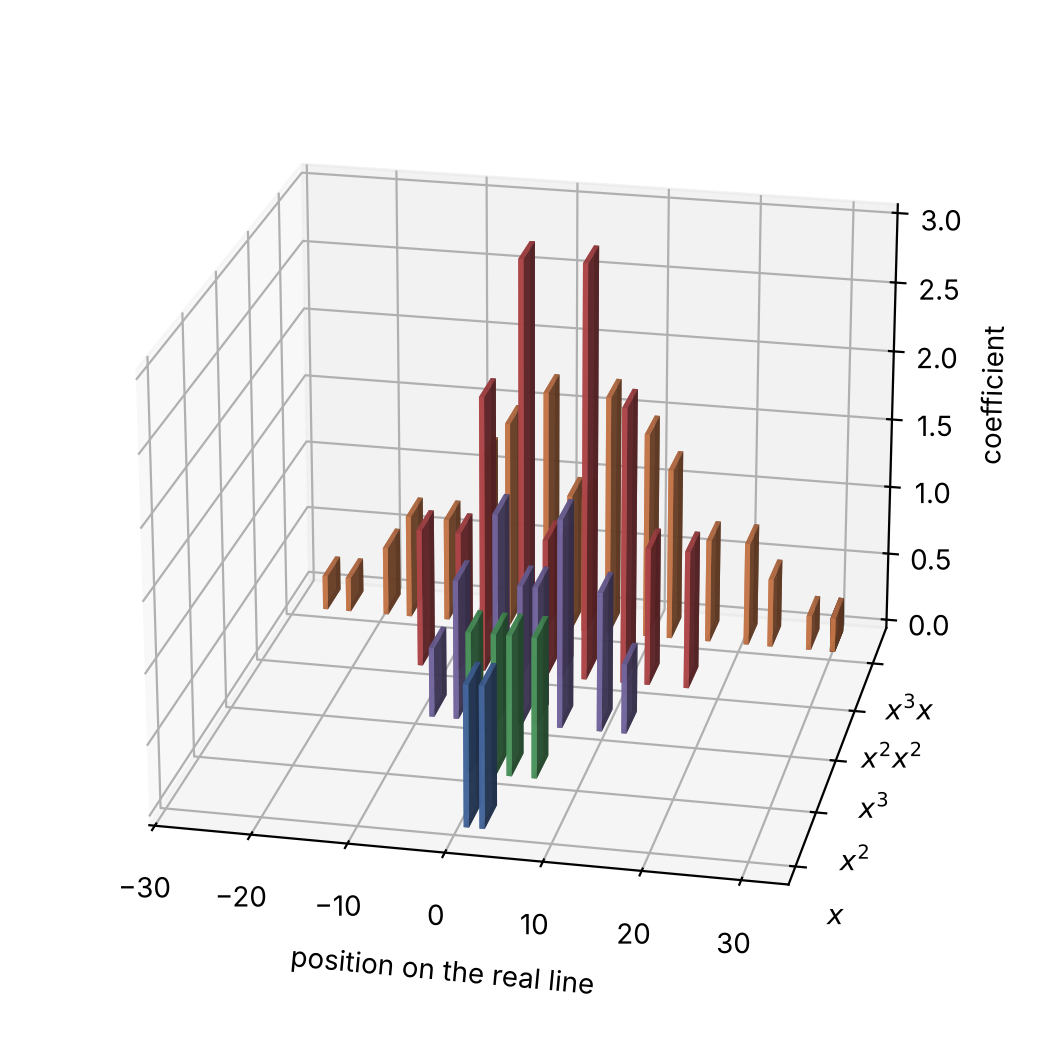
\includegraphics[width=0.82\textwidth]{fig_supports.png}
\caption{Supports and coefficients of $x$, $x^2$, $x^3$, $x^2x^2$ and $x^3x$ for $x=L_1+L_{1+\tau}$ in $\J(\mathcal F_{1,0})$, plotted at the positions of the points on the real line. The rightmost bar of $x^3x$ is $L_{9+13\tau}\approx L_{30.03}$ with coefficient $\frac14$; the support of $x^2x^2$ ends at $5+7\tau\approx16.33$.}
\label{fig:supports}
\end{figure}

\section{Finite truncations: proof of Theorem B}

For a finite subset $S\subset\Xi$ let $\pi_S$ be the linear map that keeps $L_z$ for $z\in S$ and sends $L_z$ to $0$ for $z\notin S$. Let $\J_S$ be the span of $\{L_x\}_{x\in S}$ with the product
\begin{equation}\label{eq:trunc}
L_x\circ_SL_y=\tfrac12\left(\pi_SL_{x\qa y}+\pi_SL_{y\qa x}\right).
\end{equation}
This is the truncation described in \cite[Section~6]{CCAI23}, where the product is set to zero whenever a quasiaddition leaves the chosen points. One may also read that description as setting $L_x\circ_SL_y=0$ as soon as one of $x\qa y$, $y\qa x$ lies outside $S$; the second part of Theorem~B holds for both readings.

\begin{proof}[Proof of Theorem B]
\emph{The three-point truncation.} Let $S=\{1,1+\tau,2+2\tau\}$, three consecutive points of $\mathcal F_{1,0}$, and put $e_1=L_1$, $e_2=L_{1+\tau}$, $e_3=L_{2+2\tau}$. By Lemma~\ref{lem:qa}(a), $e_i\circ_Se_i=e_i$. Example~\ref{ex:fibonacci} gives $1\qa(1+\tau)=-\tau\notin S$ and $(1+\tau)\qa1=2+2\tau\in S$, so $e_1\circ_Se_2=\frac12e_3$. Further
\begin{align*}
1\qa(2+2\tau)&=\tau^2-2\tau-2\tau^2=-1-3\tau,\\
(2+2\tau)\qa1&=2\tau^2+2\tau^3-\tau=4+5\tau,\\
(1+\tau)\qa(2+2\tau)&=\tau^2+\tau^3-2\tau-2\tau^2=-\tau,\\
(2+2\tau)\qa(1+\tau)&=2\tau^2+2\tau^3-\tau-\tau^2=3+4\tau,
\end{align*}
and none of these lies in $S$, so $e_1\circ_Se_3=e_2\circ_Se_3=0$. For $x=e_1+e_2$ this gives
\begin{align*}
x\circ_Sx&=e_1+e_2+2\cdot\tfrac12e_3=e_1+e_2+e_3,\\
(x\circ_Sx)\circ_S(x\circ_Sx)&=e_1+e_2+e_3+2\cdot\tfrac12e_3=e_1+e_2+2e_3,\\
(x\circ_Sx)\circ_Sx&=e_1+\tfrac12e_3+\tfrac12e_3+e_2=e_1+e_2+e_3,\\
\bigl((x\circ_Sx)\circ_Sx\bigr)\circ_Sx&=e_1+e_2+e_3,
\end{align*}
the last line because $(x\circ_Sx)\circ_Sx=x\circ_Sx$. The difference of the second and fourth lines is $e_3$.

\emph{Large truncations.} Let $x\in\J(\Xi)$ have at least two points in its support. For $u,v\in\J(\Xi)$ write $P(u,v)=\{s\qa t,\ t\qa s:s\in\supp u,\ t\in\supp v\}$, a finite set containing $\supp(u\circ v)$ by \eqref{eq:uv}, and let
\[
T=\supp x\cup P(x,x)\cup P(x^2,x)\cup P(x^2,x^2)\cup P(x^3,x),
\]
the products being taken in $\J(\Xi)$. Let $S\supseteq T$ be finite. In each of the four products $x\circ x$, $x^2\circ x$, $x^2\circ x^2$, $x^3\circ x$, every quasiaddition that occurs in \eqref{eq:uv} lands in $T\subseteq S$, so under either reading of the truncation no term is removed, and the products computed in $\J_S$ coincide with those computed in $\J(\Xi)$. By Theorem~A they violate $x^2x^2=x^3x$. When $\Xi=\mathcal F(\Omega)$ is a Fibonacci chain, $T$ is a finite subset of the discrete set $\Xi\subset\R$, so every set of consecutive points of the chain that reaches from $\min T$ to $\max T$ contains $T$.
\end{proof}

Theorem~B removes the finite-dimensional algebras that \cite[Section~6]{CCAI23} proposes to feed into Svinolupov's classification \cite{Svi91}: that classification concerns structure constants of Jordan algebras, and these truncations are not Jordan algebras.

\section{Ideals, units and subalgebras: proof of Theorem C}

\begin{proof}[Proof of Theorem C(a)]
In \cite[Section~5]{CCAI23} the generators of $\J(\mathcal F_{1,0})$ are indexed by $n\in\Z$ through the $n$-th point of the chain, so that their $L_0$, $L_1$, $L_3$ are our $L_1$, $L_{1+\tau}$, $L_{2+3\tau}$, and $\mathfrak k=\{L_1\circ u:u\in\J(\mathcal F_{1,0})\}$. By \eqref{eq:uv}, every element of $\mathfrak k$ is a combination of generators $L_{1\qa y}$ and $L_{y\qa1}$ with $y\in\mathcal F_{1,0}$. The generator $L_{1+\tau}$ is not among them: $1\qa y=1+\tau$ means $\tau^2-\tau y=\tau^2$, so $y=0$; and $y\qa1=1+\tau$ means $\tau^2y=1+2\tau=\tau^3$, so $y=\tau$; neither $0$ nor $\tau$ belongs to $\mathcal F_{1,0}$. So the coefficient of $L_{1+\tau}$ vanishes on $\mathfrak k$. On the other hand, by Example~\ref{ex:fibonacci}, $L_1\circ L_{1+\tau}=\frac12(L_{-\tau}+L_{2+2\tau})\in\mathfrak k$, and
\begin{align*}
(-\tau)\qa(2+3\tau)&=-\tau^3-2\tau-3\tau^2=-4-7\tau,\\
(2+3\tau)\qa(-\tau)&=2\tau^2+3\tau^3+\tau^2=6+9\tau,\\
(2+2\tau)\qa(2+3\tau)&=2\tau^2+2\tau^3-2\tau-3\tau^2=1+\tau,\\
(2+3\tau)\qa(2+2\tau)&=2\tau^2+3\tau^3-2\tau-2\tau^2=3+4\tau,
\end{align*}
so that
\[
(L_1\circ L_{1+\tau})\circ L_{2+3\tau}=\tfrac14\left(L_{-4-7\tau}+L_{6+9\tau}+L_{1+\tau}+L_{3+4\tau}\right),
\]
whose coefficient of $L_{1+\tau}$ is $\frac14$. Hence $\mathfrak k\circ\J(\mathcal F_{1,0})\not\subseteq\mathfrak k$.
\end{proof}

\begin{proof}[Proof of Theorem C(b)]
Let $\varepsilon\bigl(\sum a_xL_x\bigr)=\sum a_x$. By \eqref{eq:product}, $\varepsilon(L_x\circ L_y)=1=\varepsilon(L_x)\varepsilon(L_y)$, so $\varepsilon$ is an algebra homomorphism onto $\R$. Its kernel is an ideal; it is proper because $\varepsilon(L_x)=1$, and nonzero because it contains $L_a-L_b$ for distinct $a,b\in\Xi$. So $\J(\Xi)$ is not simple.
\end{proof}

\begin{proof}[Proof of Theorem C(c)]
\emph{No unit.} Let $I=\sum\xi_xL_x$ satisfy $I\circ L_s=L_s$ for all $s\in\Xi$. By \eqref{eq:uv}, $I\circ L_s=\frac12\sum_x\xi_x(L_{x\qa s}+L_{s\qa x})$, and by Lemma~\ref{lem:qa}(c) the generator $L_s$ occurs in $L_{x\qa s}+L_{s\qa x}$ only for $x=s$, where it occurs twice. So the coefficient of $L_s$ in $I\circ L_s$ is $\xi_s$, and $\xi_s=1$ for every $s\in\Xi$. Since $\Xi$ is infinite by Lemma~\ref{lem:qa}(d), this contradicts the finiteness of $\supp I$.

\emph{Squares grow.} Let $u\in\J(\Xi)$ have at least two points in its support, choose $f$ as in the proof of Theorem~A, and let $u_0=u$, $u_{k+1}=u_k\circ u_k$. By Lemma~\ref{lem:square} and induction, every $u_k$ is $f$-sharp with $M_f(u_k)>m_f(u_k)$ and $M_f(u_{k+1})>M_f(u_k)$. The highest point of $u_k$ therefore has a larger value of $f$ than every point in the supports of $u_0,\dots,u_{k-1}$, so $u_0,u_1,u_2,\dots$ are linearly independent.

\emph{Subalgebras.} If $\R u$ is a subalgebra with $u\ne0$, then $u_1=u\circ u\in\R u$, so $u$ cannot have two points in its support, since then $u_0,u_1$ would be independent; hence $u=cL_x$, and conversely $\R L_x$ is a subalgebra because $L_x\circ L_x=L_x$. If $B$ is a subalgebra of dimension at least two, it contains an element with at least two points in its support: take independent $v,w\in B$; if neither has two points in its support, then $v=cL_s$ and $w=dL_t$ with $s\neq t$, and $v+w\in B$ has two. That element generates the infinite independent family $u_0,u_1,\dots$ inside $B$, so $B$ is infinite-dimensional.
\end{proof}

\begin{proof}[Proof of Theorem C(d)]
A subalgebra of a Jordan algebra satisfies the Jordan identity, and $\J(\Xi)$ does not, by Theorem~A. The extension of \cite[Section~5]{CCAI25} is $\J(\Xi)\oplus\R$ with a product that restricts to \eqref{eq:product} on $\J(\Xi)$, as stated there, so it is not a Jordan algebra.
\end{proof}

\section*{Declarations}

\noindent\textbf{Data availability.} All results are proved in the text. A script that rechecks in exact arithmetic the finite computations of Example~\ref{ex:fibonacci}, Theorem~B and Theorem~C(a) is included with the source files of this paper (file \texttt{anc/verify\_jordan.py}) and archived, with the \LaTeX{} source, at Zenodo, \doi{10.5281/zenodo.24123095}.

\noindent\textbf{Funding.} This research received no external funding.

\noindent\textbf{Conflict of interest.} The author declares no conflict of interest.

\noindent\textbf{Ethics.} Not applicable.

\emergencystretch=2em
\begin{thebibliography}{99}

\bibitem{Alb48} A.~A.~Albert, \emph{Power-associative rings}, Trans. Amer. Math. Soc. \textbf{64} (1948), 552--593, \doi{10.1090/S0002-9947-1948-0027750-7}.

\bibitem{Arch} D.~Bhattacharjee, \emph{The brane cohomology conjecture for exceptional super Yang--Mills is false}, Zenodo, 2026, \doi{10.5281/zenodo.24122696}.

\bibitem{BM94} S.~Berman and R.~V.~Moody, \emph{The algebraic theory of quasicrystals with five-fold symmetries}, J. Phys. A: Math. Gen. \textbf{27} (1994), 115--129, \doi{10.1088/0305-4470/27/1/007}.

\bibitem{Bha22} D.~Bhattacharjee, \emph{Establishing equivariant class $[O]$ for hyperbolic groups}, Asian Res. J. Math. \textbf{18} (2022), no.~11, 362--369, \doi{10.9734/arjom/2022/v18i11615}.

\bibitem{Bha26} D.~Bhattacharjee, \emph{Residual-dimension obstructions for null-projected supersymmetric Yang--Mills theories}, Preprints.org, 2026, \doi{10.20944/preprints202610.3127.v1}.

\bibitem{Bha26b} D.~Bhattacharjee, \emph{Homotopy groups of spheres, Hopf fibrations and Villarceau circles II: advances in fiber bundle topology and spherical homotopy theory}, Preprints.org, 2026, \doi{10.20944/preprints202602.2038.v1}.

\bibitem{CCAI23} D.~Corradetti, D.~Chester, R.~Aschheim and K.~Irwin, \emph{Three Fibonacci-chain aperiodic algebras}, Quaest. Math. \textbf{46} (2023), no.~12, 2475--2487, \doi{10.2989/16073606.2023.2178984}.

\bibitem{CCAI25} D.~Corradetti, D.~Chester, R.~Aschheim and K.~Irwin, \emph{Jordan algebras over icosahedral cut-and-project quasicrystals}, J. Geom. Phys. \textbf{217} (2025), 105645, \doi{10.1016/j.geomphys.2025.105645}.

\bibitem{McC04} K.~McCrimmon, \emph{A Taste of Jordan Algebras}, Universitext, Springer, New York, 2004, \doi{10.1007/b97489}.

\bibitem{PPT98} J.~Patera, E.~Pelantov\'a and R.~Twarock, \emph{Quasicrystal Lie algebras}, Phys. Lett. A \textbf{246} (1998), 209--213, \doi{10.1016/S0375-9601(98)00495-2}.

\bibitem{Svi91} S.~I.~Svinolupov, \emph{Jordan algebras and generalized Korteweg--de Vries equations}, Theoret. and Math. Phys. \textbf{87} (1991), 611--620, \doi{10.1007/BF01017947}.

\end{thebibliography}

\end{document}
